% =========================================================
% 13. DATA COLLECTION - WALKING & STANDING
% =========================================================

\begin{frame}{13. How the Data Was Collected: Walking \& Standing}
\subtitleline{Left: measured CSI amplitude for that take. Right: the activity being performed.}

\vspace{-0.05cm}

% ---------------- ROW 1 : WALKING ----------------
\begin{tikzpicture}
\node[rounded corners=4pt,fill=LightOrange,inner xsep=8pt,inner ysep=3pt]
{\small\bfseries\color{AmritaMaroon}Walking};
\end{tikzpicture}
{\scriptsize\color{AmritaDark}\;\;action take \textperiodcentered\ Amrith \textperiodcentered\ Room A}

\vspace{0.08cm}

\begin{columns}[c,totalwidth=\textwidth]
\column{0.62\textwidth}
\centering
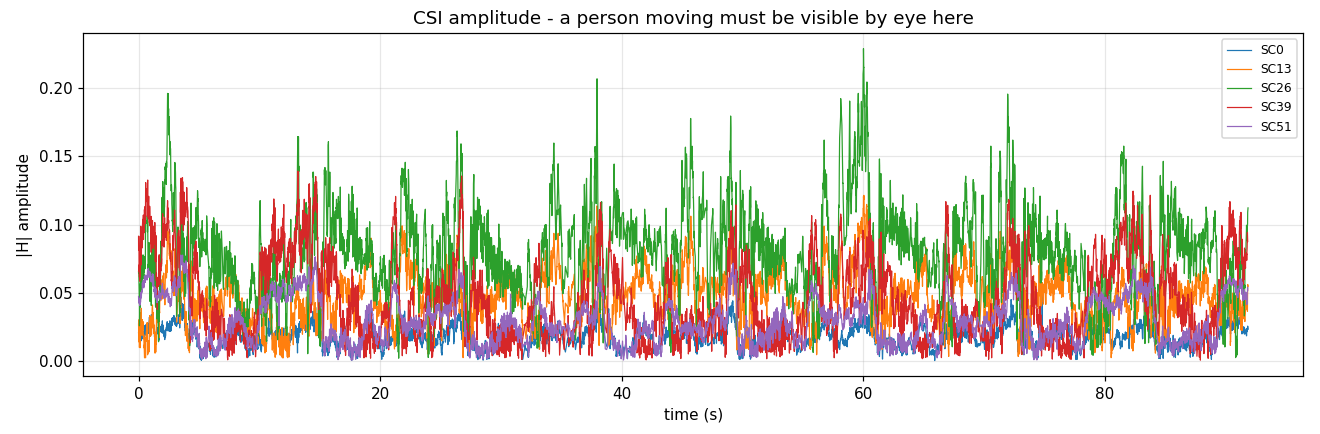
\includegraphics[height=2.5cm,keepaspectratio]{ppt_images/graph_walk.png}
\column{0.36\textwidth}
\centering
\includegraphics[height=2.5cm,keepaspectratio]{ppt_images/person_walk.jpg}
\end{columns}

\vspace{0.22cm}

% ---------------- ROW 2 : STANDING ----------------
\begin{tikzpicture}
\node[rounded corners=4pt,fill=LightBlue,inner xsep=8pt,inner ysep=3pt]
{\small\bfseries\color{AmritaMaroon}Standing};
\end{tikzpicture}
{\scriptsize\color{AmritaDark}\;\;no-action take \textperiodcentered\ Rishiikesh \textperiodcentered\ Room A}

\vspace{0.08cm}

\begin{columns}[c,totalwidth=\textwidth]
\column{0.62\textwidth}
\centering
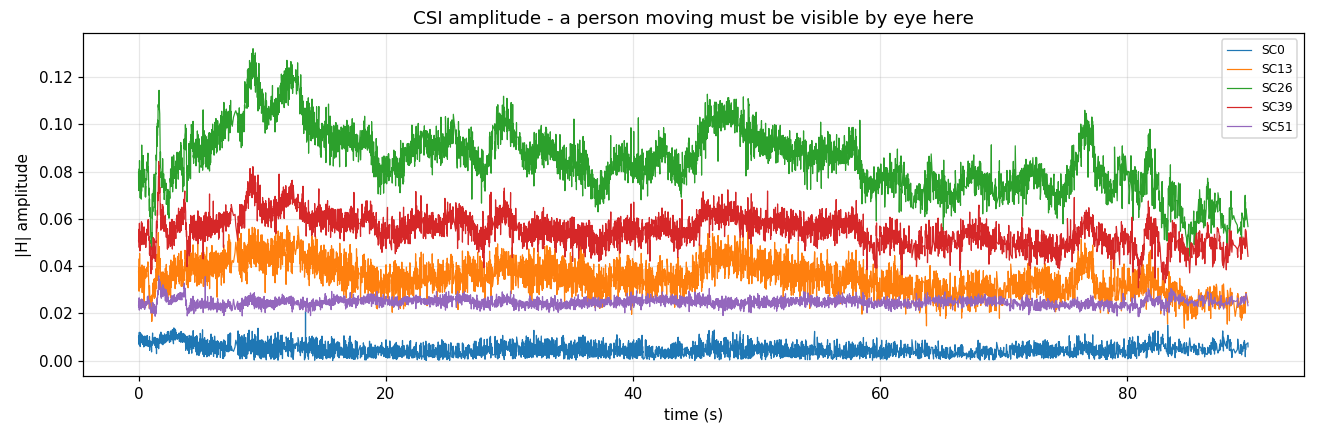
\includegraphics[height=2.5cm,keepaspectratio]{ppt_images/graph_stand.png}
\column{0.36\textwidth}
\centering
\includegraphics[height=2.5cm,keepaspectratio]{ppt_images/person_stand.jpg}
\end{columns}

\end{frame}


% =========================================================
% 14. DATA COLLECTION - SITTING & MIXED ACTIVITY
% =========================================================

\begin{frame}{14. How the Data Was Collected: Sitting \& Mixed Activity}
\subtitleline{Left: measured CSI amplitude for that take. Right: the activity being performed.}

\vspace{-0.05cm}

% ---------------- ROW 1 : SITTING ----------------
\begin{tikzpicture}
\node[rounded corners=4pt,fill=LightBlue,inner xsep=8pt,inner ysep=3pt]
{\small\bfseries\color{AmritaMaroon}Sitting};
\end{tikzpicture}
{\scriptsize\color{AmritaDark}\;\;no-action take \textperiodcentered\ Rishiikesh \textperiodcentered\ Room A}

\vspace{0.08cm}

\begin{columns}[c,totalwidth=\textwidth]
\column{0.62\textwidth}
\centering
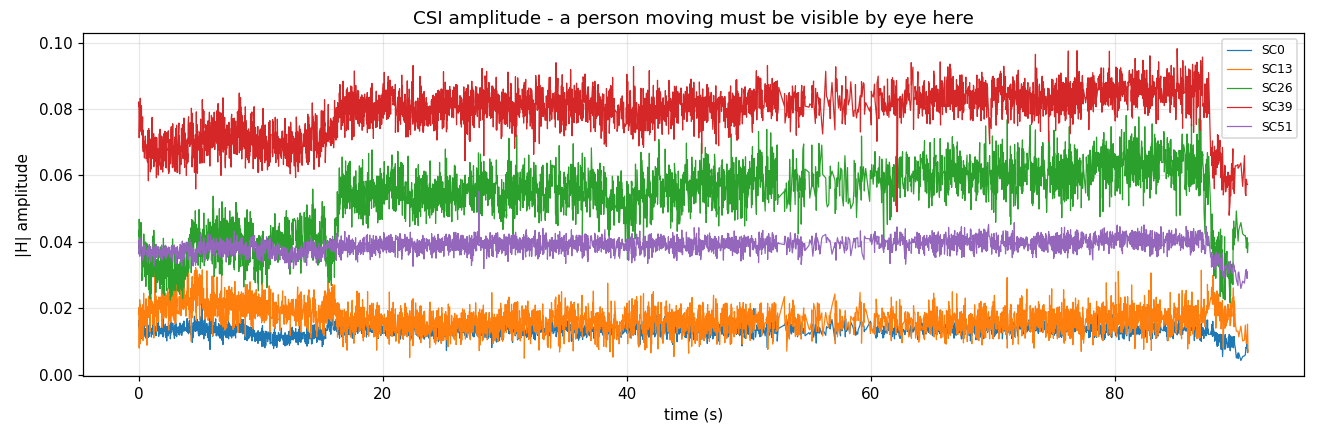
\includegraphics[height=2.5cm,keepaspectratio]{ppt_images/graph_sit.png}
\column{0.36\textwidth}
\centering
\includegraphics[height=2.5cm,keepaspectratio]{ppt_images/person_sit.jpg}
\end{columns}

\vspace{0.22cm}

% ---------------- ROW 2 : MIXED ACTIVITY ----------------
\begin{tikzpicture}
\node[rounded corners=4pt,fill=LightOrange,inner xsep=8pt,inner ysep=3pt]
{\small\bfseries\color{AmritaMaroon}Mixed activity};
\end{tikzpicture}
{\scriptsize\color{AmritaDark}\;\;action take \textperiodcentered\ Gowreesh \textperiodcentered\ Room B}

\vspace{0.08cm}

\begin{columns}[c,totalwidth=\textwidth]
\column{0.62\textwidth}
\centering
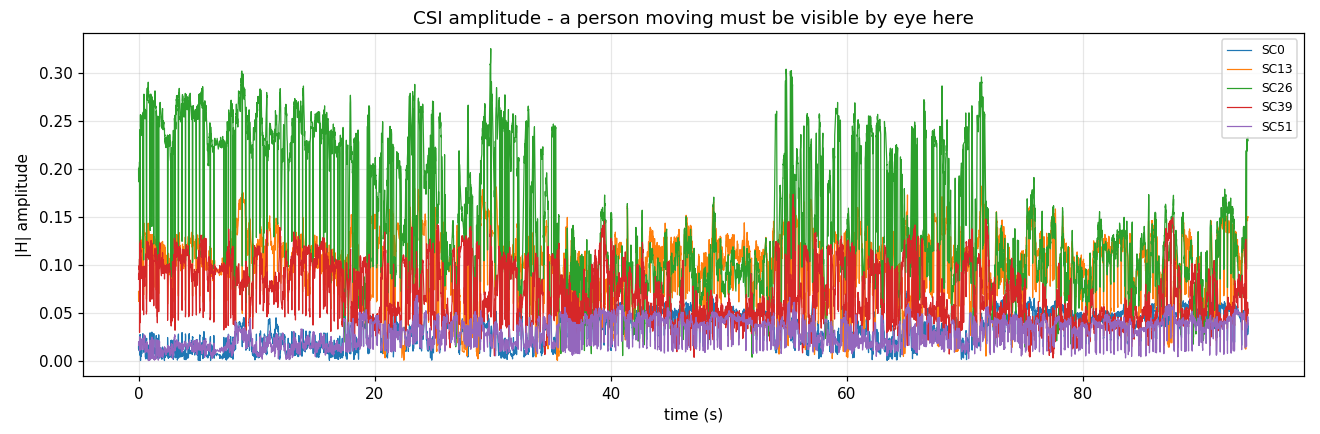
\includegraphics[height=2.5cm,keepaspectratio]{ppt_images/graph_mixed.png}
\column{0.36\textwidth}
\centering
\includegraphics[height=2.5cm,keepaspectratio]{ppt_images/person_mixed.jpg}
\end{columns}

\end{frame}
